\chapter{GPU微体系结构研究}\label{chap:GPUArch}
对GPU微体系结构的研究一直是高性能计算领域的一个热点。人们对传统的x86和ARM CPU微架构已经有了较为详尽的理解。研究人员利用GEM5CPU模拟器进行处理器微结构的设计和研究,但当前针对GPU的模拟器还十分落后于工业界。因此对GPU微结构的理解可以帮助研究人员设计出更加真实的GPU模拟器,同时也使得编程人员可以设计出高效的GPU程序。
\section{OpenCL编程模型}
OpenCL(Open Computing Language)既是一个语言,也是一个标准,OpenCL用于异构编程领域。对于AMD GPU,OpenCL是其主要编程语言之一。

\subsection{OpenCL程序语言介绍}
OpenCL是一种异构并行编程语言,OpenCL标准最初由苹果公司提出,同时参与的公司有AMD,IBM,Qualcomm,Intel和NVIDIA。最后由Khronos Group进行标准化和发布。Khronos Group在2008年发布了OpenCL标准的第一版,OpenCL 1.0。OpenCL 1.0定义了主机端的编程接口和设备端的编写kernel的语言。OpenCL语言基于C语言发展而来。随后发布的OpenCL 1.1和1.2标准增加了OpenCL与OpenGL的互操作性。在2013年,正式发布了OpenCL 2.0标准。新标准在一定程度上简化了并行程序的开发。OpenCL的API在设计上就做的尽可能通用,以使其可以运行在不同的平台上;并且也足够底层,以使其可以在不同的平台上都可以获得较高的性能。

OpenCL程序在不同的平台具有可移植性,按照OpenCL标准编写的程序,可以在不同的硬件平台上运行。用OpenCL C语言可以编写在OpenCL设备上运行程序。OpenCL C在C99的基础上发展而来。其设计的目标是可在不同的OpenCL硬件平台(如GPU、FPGA、DSP等)上编写并执行可数据并行的程序。同时OpenCL C也实现了一组原子和同步操作。虽然OpenCL API本身是基于C的API,但也可以绑定到其他语言,例如Python,C++,Java等。另外,很多专用的库如数学库,计算机视觉库)也都集成了OpenCL的实现,来提升异构系统的计算性能。所以,我们可以看到OpenCL的目标是做通用并行计算。OpenCL 标准包含4部分,分别是平台模型,执行模型,kernel编程模型和内存模型。

平台模型:在OpenCL平台模型中,有一个主机端和一到多个设备端。主机端用来协调OpenCL代码的执行,设备端执行kernel代码。平台模型提供了一个抽象的硬件设备模型。

执行模型:执行模型定义了主机端OpenCL环境的配置和kernel的调用。这里包括OpenCL执行环境的配置,主机端与设备端的交互配置和kernel并发模型的配置。并发模型定义了如何kernel的执行分解到的线程和线程块这样的并行粒度。

Kernel编程模型:描述了如何将并发模型映射到具体的物理设备
内存模型:描述了kernel执行时使用的抽象内存层次结构,而不管具体的物理内存结构。

一个x86 CPU和GPU构成了常见的OpenCL硬件环境。其中CPU作为主机端,GPU作为加速器。使用执行模型,我们在主机端对 kernel进行配置,指定kernel执行时的并行粒度,并向GPU发出执行kernel的命令。我们在给GPU端的数据分配内存时,按照内存模型中的抽象内存层次来进行分配。OpenCL运行时和驱动将抽象的内存区域映射到具体的物理内存层次中。最后,使用kernel编程模型,GPU创建硬件线程来执行kernel;GPU进行调度时,线程会映射到具体的计算单元来执行。

一个通用的OpenCL设备包含多个CUs(Compute Units),每个CU每个最终由多个ALUs构成。一个线程(或者SPMD(单程序多数据)kernel的一个执行实例)最终会执行在一个ALU上。

对于AMD Radeon Instinct MI25(Vega10)和AMD Radeon Instinct MI8(Fiji)架构的GPU,每颗芯片有64个CUs,对于AMD Radeon Instinct MI6(Polaris)架构,每颗芯片有32个CUs。其中,每个CU包含一个标量单元和四个向量单元。每个向量单元是一个宽度为16的向量ALU。这四个向量单元以SIMD的方式执行指令。在单个CU上可以同时执行多个wavefronts。
\begin{figure}[htbp]
	\centering
	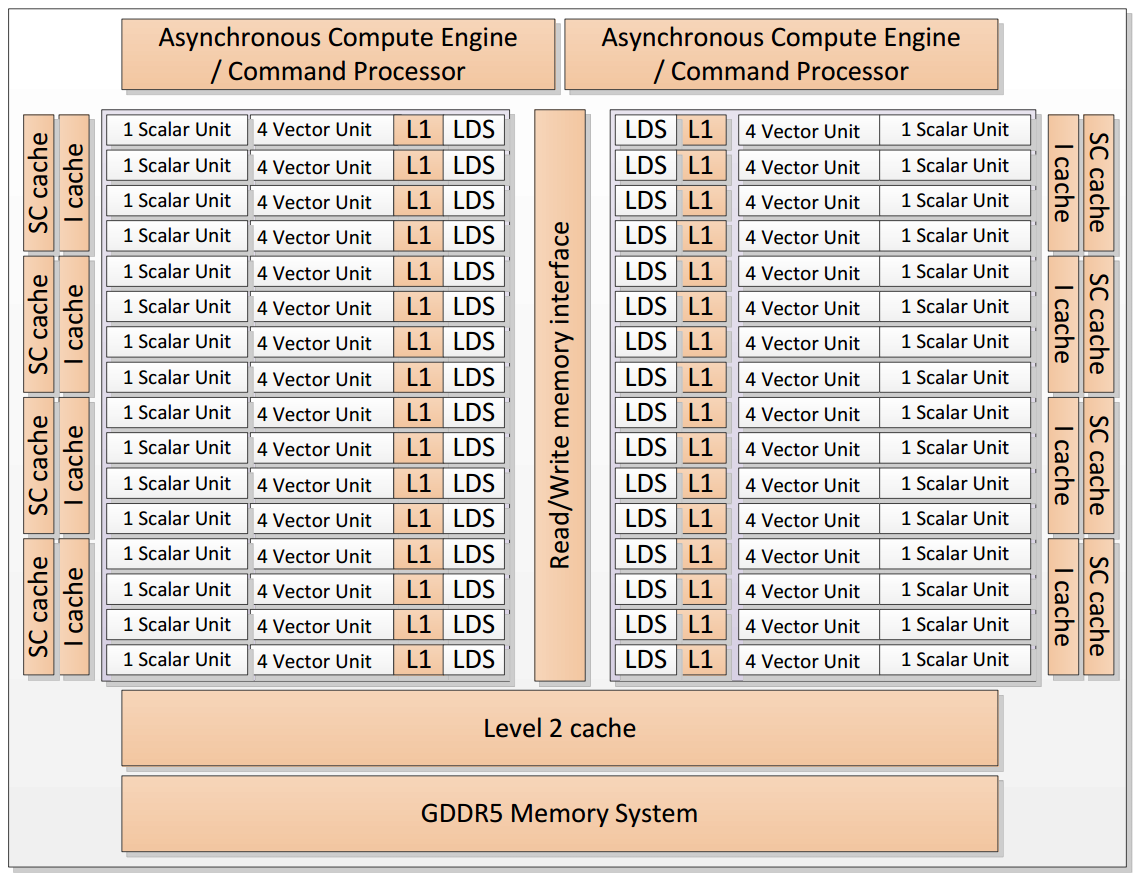
\includegraphics[width=0.50\textwidth]{gcn_gpu}
	\bicaption{GCN GPU结构图}{GCN GPU architecture}
	\label{fig:gcn_gpu}
\end{figure}
在AMD GCN架构中,一个CU包含一个标量单元和四个向量单元,一个L1 cache和一个LDS(Local Data Share)。在程序指令流中,既有标量指令也有向量指令。在每个时钟周期,指令调度器会选择一个标量指令和一个向量指令(或者访存指令,分支指令),分别发射到标量单元和向量单元。


\subsection{AMD ROCm软硬件系统}
本文主要针对AMD GPU架构做分析和性能调优。所以,我们就介绍AMD GPU的OpenCL实现。AMD APP(Accelerated Parallel Processing)是AMD最先提出的并行加速处理概念。AMD APP利用AMD GPU强大的处理能力来做高性能计算和数据并行处理。AMD ROCm系统包含AMD GPU、AMD多核CPU和与之相关的软件栈。图\ref{fig:rocm_llvm}是AMD ROCm编译工具链。
\begin{figure}[htbp]
	\centering
	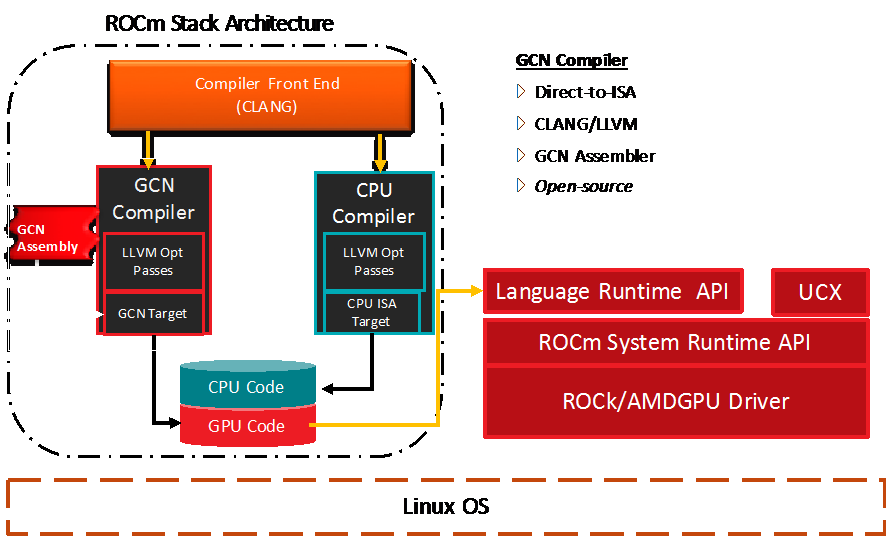
\includegraphics[width=0.50\textwidth]{rocm_llvm}
	\bicaption{AMD ROCm编译工具链}{AMD ROCm Compilation Tool Chain}
	\label{fig:rocm_llvm}
\end{figure}

AMD ROCm软件栈为用户和软件开发人员提供完整,灵活的软件开发工具来提升AMD GPU处理器的计算性能。AMD ROCm软件栈是一个开放的系统和一个标准的平台。AMD ROCm开放平台的策略让AMD的技术合作伙伴可以开发和提供第三方开发工具。

AMD ROCm提供的工具包括:

(1) OpenCL编译器和运行时。

(2) 调试和性能分析工具----AMD CodeXL。

(3) 高性能数学库(rocBLAS, Tensile)---AMD加速并行处理数学库,用于优化NDRange特定算法。

最新的AMD GPUs使用同一着色器架构可以在相同的硬件上交替运行不同的kernel。可编程GPU可以执行不同的用户程序,这些程序对图形编程人员称之为shaders,对于做通用计算的人称之为kernels。这些GPUs计算设备可以使用数据并行编程模型做通用计算,而不做图形渲染。AMD ROCM的编程模型将一组数据存放在内存中,这些数据可以被大量的计算单元(Compute Units)所访问。

\subsection{OpenCL线程模型}
Kernel的每个实例运行在Compute Unit(以下简称CU)上,称为work-item。work-items被映射到一个N维的索引空间,称为NDRange。图\ref{fig:opencl_thread_model}展示了AMD OpenCL线程模型和线程到CU的映射关系。
\begin{figure}[htbp]
	\centering
	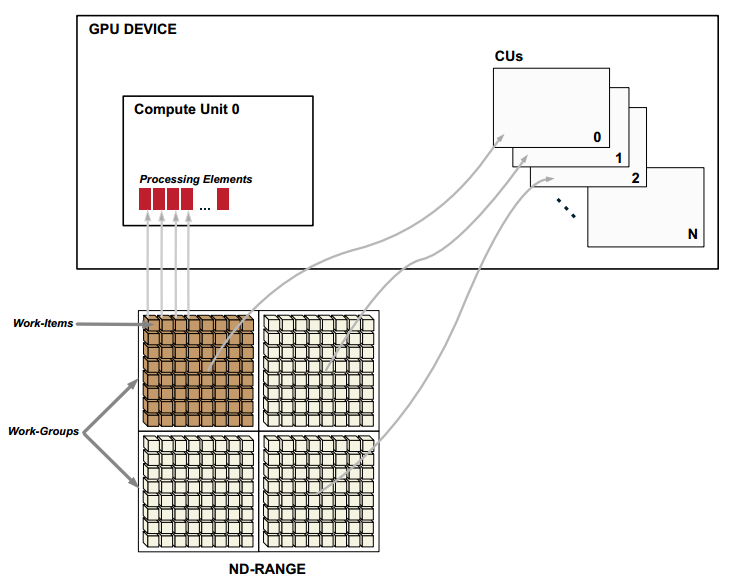
\includegraphics[width=0.50\textwidth]{opencl_thread_model}
	\bicaption{AMD OpenCL线程模型}{AMD OpenCL thread model}
	\label{fig:opencl_thread_model}
\end{figure}

一个work-group被分发到某一个CU上。Work-group中的work-item被一个CU中PE(Processing Element)所处理。一个PE在同一时刻只能处理一个work-item;但一个CU可以处理多个work-group。OpenCL将所有要发射的线程映射到一个N维的索引空间。软件开发人员可以设定如何将work-items划分到work-group中。AMD GPU硬件调度的基本单元是wavefront,一个wavefront有64个线程(work-items)。一个work-group由整数倍个wavefront构成。图\ref{fig:thread_model}展示了work-item,wavefront和NDRange之间的映射关系。
\begin{figure}[htbp]
	\centering
	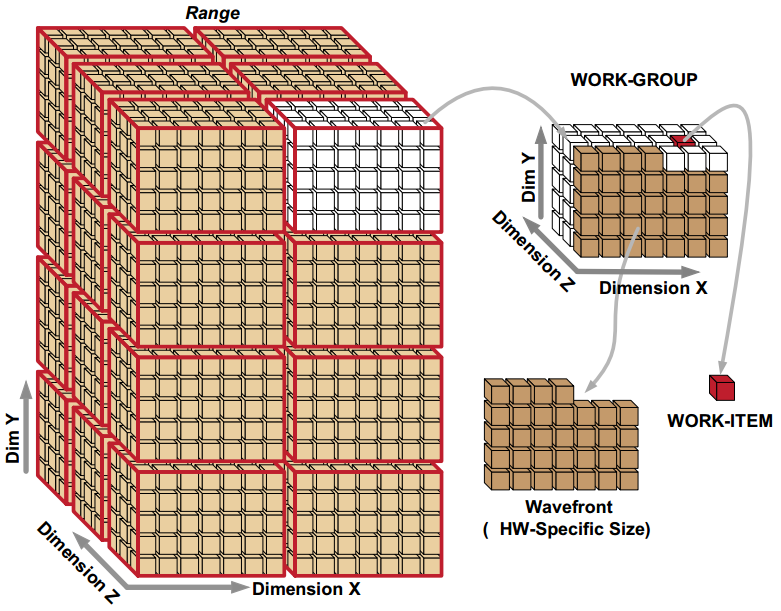
\includegraphics[width=0.50\textwidth]{thread_model}
	\bicaption{OpenCL线程组织方式}{OpenCL thread organization}
	\label{fig:thread_model}
\end{figure}

其中,wavefront是硬件上的概念,即AMD GPU硬件设计上的64个线程为一个基本调度单元。Work-group和NDRange是编写程序时的逻辑概念。一个work-item在每个时钟周期会发射一条指令。多个work-item构成一个wavefront,作为一个基本调度单元。一个wavefront中至多有4个work-item组成流水线执行,来隐藏访存和计算延迟。例如,AMD GCN架构的GPU的实际处理宽度是16。每4个时钟周期发射一个宽度为64的指令。wavefront拥有的线程数在不同系列的GPUs上会有不同。例如,一些低端GPUs,如AMD Radeon HD54XX系列的GPU,一个wavefront有32个线程。在更新的高端GPUs上,一个wavefront有64个线程。每个CU的执行相互独立,在不同的CU上可以执行不同的指令。

下面讨论一下wavefront和work-group的关系。编程人员定义一个work-group,可以包含一到多个wavefronts。一个wavefront有自己的程序计数器(PC),所以每个wavefront都有自己的程序控制流。一个work-group包含的wavefront中的线程是线性排序的。例如,在64线程wavefront的GPUs上,线程0$\sim$63映射到wavefront0,线程64$\sim$127映射到wavefront1,按这样的顺序映射下去。为了充分利用硬件资源,要计算的数据个数最好是64的整数倍。

对于每个work-group,GPU会在单个CU上产生该work-group所需的wavefronts个数。如果一个wavefront中有非活跃的线程,那么这些线程所映射的GPU硬件计算核心将会空闲。出现这种情况的一个例子是我们的work-group的大小不是wavefront大小的整数倍。例如,如果一个work-group的大小是32,只使用了wavefront中的一半线程,那么就会有另外32个线程空闲。

在一个wavefront中,如果程序出现分支,wavefront将会把有所的情况组合起来,顺序的执行。例如,一个wavefront中的一个分支包含两条路径,那么wavefront会先执行第一条路径,接下来执行第二条路径。分支的总执行时间是每个路径的执行时间的累加。例如,程序中有一个二分支结构,分支A和B,每个分支单独执行所需的时间都是t。只要wavefront中有一个线程在分支处和其他线程不同,那么整个wavefront执行完这段分支的时间就是2t。我们再举一个循环的例子,如果一个循环的单次执行时间是t。在一个wavefront中,有63个线程只执行这个循环的一次,另外一个线程执行该循环100次。那么整个wavefront执行完该循环的时间为100t。

OpenCL编译工具链提供了一个可以同时编译CPUs和GPUs代码的通用框架。CPUs和GPUs代码共用编译器前端和部分高级的编译转换。编译器后端则针对不同的设备(CPU或GPU)做了专门的优化。对于CPU,OpenCL运行时使用LLVM AS将代码编译成x86二进制代码。OpenCL运行时会自动确定CPU的核心数,并将OpenCL kernel交由核心执行。对于GPU,OpenCL运行时对不完整的AMD IL做后处理,变成完整的AMD IL。这个过程会从宏定义库中添加针对特定GPU的宏定义。之后,OpenCL运行时会移除不必要的函数,将完整的IL代码交由着色器编译器,编译成针对特定GPU的二进制代码。

%平台模型:
%
%OpenCL平台包含一个主机端和一到多个OpenCL设备。一个OpenCL设备包含一到多个CUs(Compute Units),一个CU包含一到多个PEs(Processing Elements)。

%平台模型是开发可在不同硬件平台上运行的程序的一个关键。在一个系统中,可能同时包含AMD GPU和NVIDIA GPU。

编程人员可以使用平台模型API来选择平台和计算设备。平台模型提供了一个抽象的设备体系结构,编程人员可以根据这个抽象体系结构来编写kernel。硬件厂商会将这个抽象体系结构映射到具体的物理硬件上。平台模型将设备定义为一组CUs(Compute Units),每个CU相对独立。每个CU由一组PEs(Processing Elements)组成。以2017年AMD新出Vega10架构为例,Vega10计算卡包含64个CUs,每个CU包含4个宽度为16的SIMD部件,所以一个CU的硬件向量宽度为64。由此可以计算出一张Vega10计算卡可以一次总共执行64x16x4=4096个指令。再根据Vega10的计算时钟频率最大为1.5GHz,每个时钟周期可以做2个浮点操作,可以计算出Vega10的理论单精度浮点峰值为64x16x4x2x1.5GHz=12288.0 Gflop/s。
%获取平台和设备信息:
%
%我们可以调用clGetPlatformIDs()函数来获取系统的平台信息。
%
%获取了每个平台的ID号之后,我们通过调用clGetPlatformInfo()函数来获取每个平台的硬件厂商信息。
%
%当我们选好平台后,接下来就可以调用clGetDeviceIDs()选择该平台的一个具体设备。
%
%在本次实验中,我们的一个CPU连接两个AMD vega10 GPU。
%
%我们接下来就可以选择在该平台每个设备的ID号后,可以通过调用clGetDeviceInfo()获取该平台每个设备的信息。
%
%本次实验使用的是AMD vega10 GPU,又称gfx900。
%
%对于vega10 GPU,有64个CUs。
%
%更多信息在此就不一一列举。
%
%前面部分主要介绍了如何获取选择平台和平台上的设备,并获取平台和该平台上设备的信息。虽然看起来很冗长,但对我们理解OpenCL的平台模型很有帮助。
%
%执行模型:
%
%为了主机端可以向设备发送命令和数据,我们要创建一个context。
%
%Context介绍:
%
%在OpenCL中,context是一个抽象环境。在这个抽象环境中,我们可以协调kernel的执行和管理kernel的内存。并且可以对kernel的执行进行跟踪。
%
%OpenCL运行时(runtime)使用contexts来管理各种对象,例如命令队列(command queues),内存,程序(program)和kernel等对象;并且使用contexts中指定的设备来运行kernel。
%
%在OpenCL中,查询平台和设备信息,创建context的过程看起来很冗长。然而,当我们写好这些代码后,我们就可以在之后的项目中重用这部分代码。
%
%命令队列(command-queues):
%
%设备端执行任务的方式是,主机端向设备端发送命令(commands),设备根据该命令来执行任务。这里的命令(commands)包括执行kernel,数据传输,同步操作。
%
%主机端请求设备端执行任务,需要通过命令队列(command-queues)这种通信机制。当我们选定设备,并且创建了与选定设备关联的context之后,我们需要针对选定的每一个设备创建一个与之对应的命令队列(command-queues)。每个命令队列只能和一个设备关联。因为一个context中可能关联多个设备。在当前的context中,主机端向具体某一个设备发送命令时,就需要一个与该设备关联的命令队列。
%当主机端需要某一个设备执行某种操作时,主机端需要将相应的命令提交到对应的命令队列中。
%
%事件(Events):
%
%OpenCL中的事件是与命令的状态相关联的对象。命令队列中的命令会产生事件,其他命令在执行之前需要等待某个事件。
%设备端队列(device-side enqueuing):
%
%从另一个角度来看我们的异构计算平台。我们可以将之看成master-worker模型。在该模型中,主机端(master)发送命令给设备端(worker)。通过master-worker模型,主机端和设备端可以协作工作。然而,在很多情况下,特别是在运行有前后依赖的算法时,主机端并不能静态的确定向设备端分发的任务数。例如在组合优化中,搜索区域的大小可能会决定下次work-groups的数目。然而,搜索区域的大小只能从上一次的迭代中获知。在之前的OpenCL版本中,为了给下一次运行的kernel设置合适的并行粒度,需要设备端和主机端进行通信来确定。为了去除这样的通信要求和提高系统性能,OpenCL 2.0在执行模型中增加了设备端队列(device-side enqueuing)。
%在设备端正在执行的kernel可以将另外一个kernel放入该设备端队列。在这种情形下,我们称正在执行的kernel为父kernel,放入设备端的kernel为子kernel。当父kernel和所有子kernel都已执行完,父kernel在被标记为已完成。但父kernel和子kernel的执行可以是异步的。
%
%Kernels和OpenCL编程模型:
%
%前面介绍的执行模型是为了管理OpenCL命令的执行。OpenCL命令用来描述数据的传输和kernel的执行。OpenCL kernel是OpenCL应用中实际在设备上执行的那部分程序。和CPU上的许多并发模型类似,OpenCL kernel在语法上看起来和标准的C函数类似。这里的主要区别是OpenCL kernel有一组额外的关键字和OpenCL kernels所实现的并发模型。   
%当使用操作系统提供的线程接口编写并发程序时,我们需要考虑实际的可用物理资源(如CPU物理核数)。当我们创建的线程超过CPU硬件线程数时,就需要考虑线程创建、线程间切换所带来的开销。而当使用OpenCL编写并发程序时,我们经常需要考虑如何采用最好的并行粒度来编写并行程序。

在OpenCL中,并发的最小粒度是work-item。每个work-item执行kernel函数。OpenCL运行时将work-items映射到GPU具体硬件计算单元上。从概念上来看,这种并行方式非常类似于MapReduce中的map操作。Map操作具有其天然的并行性。也类似于OpenMP中对for循环进行数据并行。图\ref{fig:thread_map}展示了NDRange,work-group,work-item之间的对应关系。在实际计算时,通常将NDRange映射到输入数据或者输出数据。在本文的矩阵乘实现中,将NDRange映射到输出数据,即C矩阵。
\begin{figure}[htbp]
	\centering
	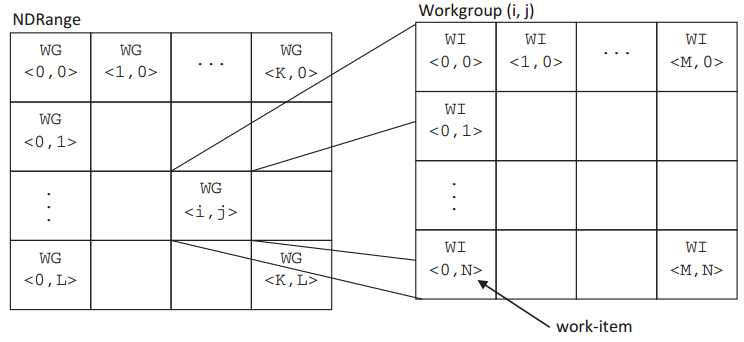
\includegraphics[width=0.50\textwidth]{thread_map}
	\bicaption{NDRange,work-group,work-item对应关系}{Relationship between NDRange, work-group and work-item}
	\label{fig:thread_map}
\end{figure}

%编译和参数处理:
%
%一个OpenCL程序可能由多个OpenCL C kernel组成。例如,在代数求解器应用中,在一个OpenCL程序中可能包含向量加,矩阵乘和矩阵转置这几个kernel。在运行时(runtime)通过一系列API调用对OpenCL源程序进行编译。运行时(runtime)编译给系统提供了针对特定计算设备进行OpenCL kernel优化的可能,也让OpenCL kernel在之前未知的OpenCL兼容的设备上运行成为可能。由于OpenCL程序运行时(runtime)编译的特性,如果我们的OpenCL程序要在AMD,NVIDIA,Intel等这些硬件厂商提供的设备上运行时,我们不需要预先针对不同硬件平台进行预编译。

创建kernel的过程:

(1) OpenCL C源程序被存储在一个字符数组中。如果源程序存放在磁盘的文件中,则将其从磁盘读取到内存,并存放在一个字符数组中。

(2) 通过调用clCreateProgramWithSource(),将OpenCL C源程序转化为程序对象 cl\_program 。

(3)	通过调用clBuildProgram(),编译程序对象。

(4)	通过调用clCreateKernel(),创建kernel对象cl\_kernel。

OpenCL kernel对象的具体二进制表示是和硬件厂商相关的。对于AMD运行时(runtime),主要有两种设备:x86CPU和GPUs。对于x86 CPU,clBuildProgram()产生可以直接在x86 CPU上执行的x86指令。对于GPU,则产生AMD GPU的中间表示语言,之后用just-in-time技术将中间语言编译成具体GPU指令集体系结构的二进制代码。图\ref{fig:opencl_model_relation}展示了OpenCL各种模型之间的关系。
\begin{figure}[htbp]
	\centering
	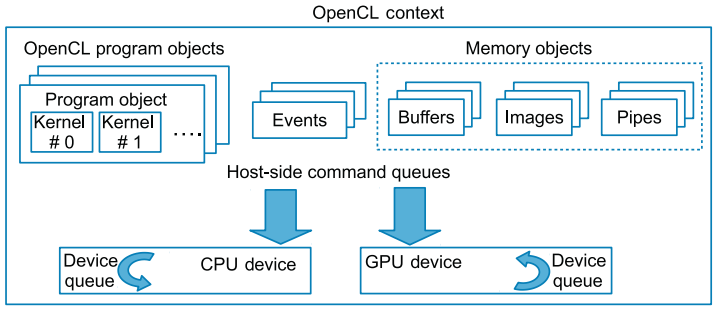
\includegraphics[width=0.50\textwidth]{opencl_model_relation}
	\bicaption{OpenCL模型之间的关系}{Relationship between OpenCL models}
	\label{fig:opencl_model_relation}
\end{figure}

NVIDIA也采用了类似的方法,将kernel代码首先编译成PTX(Parallel Thread eXecution)这种中间表示。这种中间表示的好处是可以让GPU ISA这样一代代演进,而不用考虑向后兼容的问题。因为GPU体系结构还处在一个非常快速的发展时期。

%OpenCL内存模型:
%
%不同计算设备的内存子系统会有很大不同。为了使得OpenCL代码具有可移植性,OpenCL定义了一个抽象的内存模型。编程人员可以基于该抽象内存模型来编写程序。不同的硬件厂商将此抽象内存模型映射到其具体设备的内存层次结构上。
%
%对于OpenCL kernel来说,通常我们需要向kernel传入一些参数,kernel会输出一些参数。在kernel执行前,我们要将输入数据从主机端内存拷贝到设备端内存。为了将数据从主机端拷贝到设备端,我们需要将其封装成一个内存对象。同样,对于输出数据,我们也需要将其封装成一个内存对象。OpenCL定义了三种内存对象:buffer,images和pipes。在本文的矩阵乘中,用到buffers对象,所以我们主要介绍buffer内存对象。Buffer内存对象等价于C语言中我们用malloc()分配的数组空间。

OpenCL将内存分为两部分:主机端内存和设备端内存。主机端内存和设备端内存间的数据移动通过调用相应OpenCL API完成。OpenCL设备端将内存分为4个区域。整个kernel可以访问的全局内存(Global memory)和常量内存(Constant memory),一个线程块可以访问的局部内存(Local memory),一个线程可以访问的私有内存(Private memory)。这几个内存区域在逻辑上是分离的,kernel开发人员可以显式的控制数据在这几个内存区域移动。当我们将数据从主机端拷贝到设备端时,数据就拷贝到了设备端的全局内存。也只有设备端全局内存的数据的才可拷贝回主机端的主存。局部内存通常映射到片上内存。片上内存相比全局内存延迟更低,带宽更高。每个线程的私有内存通常映射到寄存器中。

\begin{figure}[htbp]
	\centering
	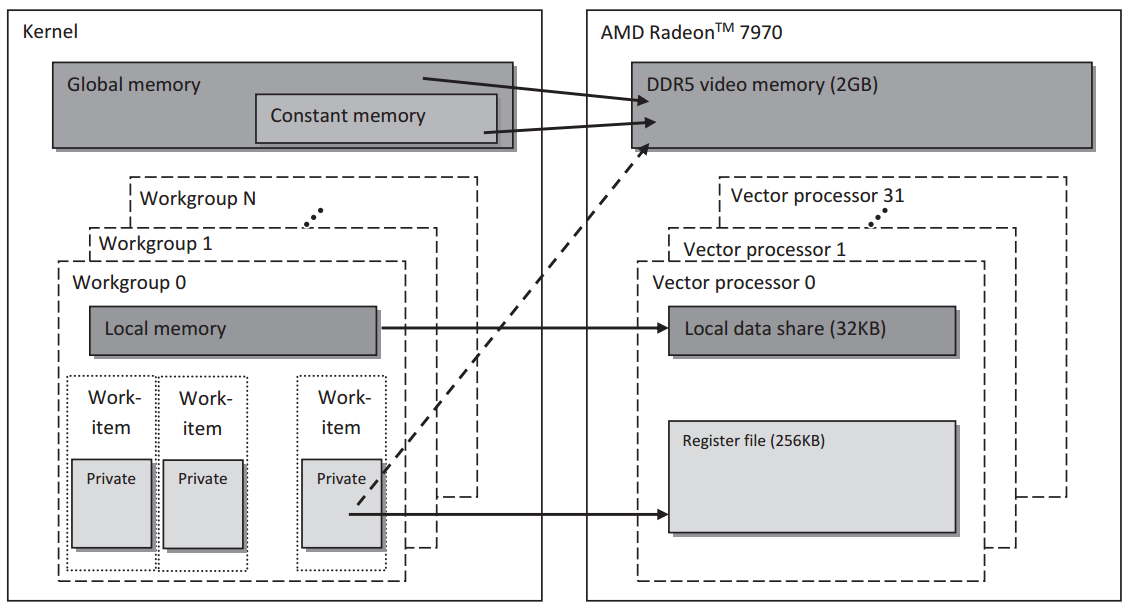
\includegraphics[width=0.50\textwidth]{opencl_memory_gpu}
	\bicaption{OpenCL内存模型与AMD GPU内存的关系}{OpenCL memory model and AMD GPU memory}
	\label{fig:opencl_memory_gpu}
\end{figure}

图\ref{fig:opencl_memory_gpu}中的虚线表示大部分情况下OpenCL中的线程私有内存对应到AMD GPU的寄存器。但也存在一些私有内存在溢出的情况下会对应到AMD GPU的片外内存。


\section{OpenCL程序在AMD GCN GPUs上的性能和调优}
接下来讨论AMD GCN(Graphics Core Next)架构GPUs上的程序性能和调优方法。AMD GCN架构的GPUs包括Fiji,Vega10和Vega20等。

\subsection{优化全局访存}
首先介绍一下GPU的组成结构,AMD GCN GPU由多个CU构成。每个CU包含局部内存(片上内存),L1 cache,寄存器和4个SIMD单元。每个SIMD包含16个计算核心。一个线程会在一个计算核心上执行,一个CU会运行一到多个work-groups。在GPUs上,硬件调度以wavefront 64个线程为基本调度单元,一个wavefront中64个线程执行相同的指令,但操作不同的数据。是一种典型的SIMD执行方式。

每个CU包含64KB的片上内存,16KB的读/写L1 cache,4个向量单元和1个标量单元。每个work-group可以最大分配32KB片上内存。每一个向量单元包含512个标量寄存器(SGPRs),用以处理一个wavefront中的分支,常量等操作。每个标量单元包含256个向量寄存器(VGPRs)。向量寄存器本质上也是标量寄存器,只是每个寄存器在长度上由1扩展到64。每个向量单元包含16个计算核心。

每个CU的L1 Cache为16KB,所以总的L1 Cache大小为$15KB\times \#CUs$。对于AMD Radeon HB7970 GPU,包含32个CUs,总共有512KB的L1 Cache。下面\ref{eq:L1bandwidth}给出L1峰值带宽的计算公式。对于AMD Radeon HD7970 GPU,由此可以计算出L1的带宽理论峰值约为$\sim$1.9TB/s。
\begin{equation}
\label{eq:L1bandwidth}
\begin{aligned}
&L1\ peak\ bandwidth = \\
&\#CUs\times (4threads/clock) \times (128 bits/thread) \times (1byte/8bits) \times Engine\ Clock
\end{aligned}
\end{equation}
%L1峰值带宽 = 
%
%\#CUs*(4threads/clock)*(128 bits/thread)*(1byte/8bits)*Engine Clock



如果两个访存请求指向同一个内存控制器,在硬件上这两个请求会顺序执行,我们称为channel冲突。与之类似,如果两个访存请求映射到同一个内存bank,那么这两个请求也会顺序执行,我们称之为bank冲突。从软件开发人员的角度来看,channel冲突和bank冲突没有太大区别。如果数据请求的步长是2的幂次方的一个较大的数,那么往往会发生channel冲突。发生冲突的步长依赖于具体的芯片。如果一个步长在有8个channel的芯片上发生channel冲突,那么这个步长也可能会在有4个bank的芯片上导致bank冲突。

在本论文中,使用bank冲突来统一指代channel冲突或bank冲突。刚才讨论到,如果访存步长是一个较大的2的幂次方的一个数,那么往往会发生channel冲突。对于CPU来说,也会遇到同样的问题,访存步长为较大的2的幂次方的一个数,会使得访问的数据落在较少的Cache lines中,产生较多的cache不命中。对于很多kernels来说,channel冲突对性能影响非常大。这时,我们就很有必要理解并解决channel冲突。在GPU程序编写中,最好的方式是安排相邻的线程来读/写相邻的内存地址,这是一种避免channel冲突的方法。图\ref{fig:gpu_mem_channel}展示了内存channel分布:
当应用程序可以完全控制数据的访存模式时,软件开发人员就需要合理的组织数据结构,使得bank冲突最小化。图\ref{fig:gpu_addr}展示了硬件地址字节分布:

\begin{figure}[htbp]
	\centering
	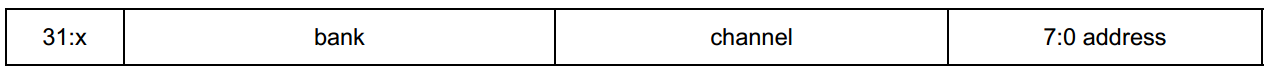
\includegraphics[width=0.80\textwidth]{gpu_addr}
	\bicaption{硬件地址字节分布}{Hardware address byte distribution}
	\label{fig:gpu_addr}
\end{figure}
Channel的计算方式:

if (({ row, bank} \%3) == 1)
channel\_within\_quadrant = 1

else

channel\_within\_quadrant = 2 * pipe[0]

\begin{figure}[htbp]
	\centering
	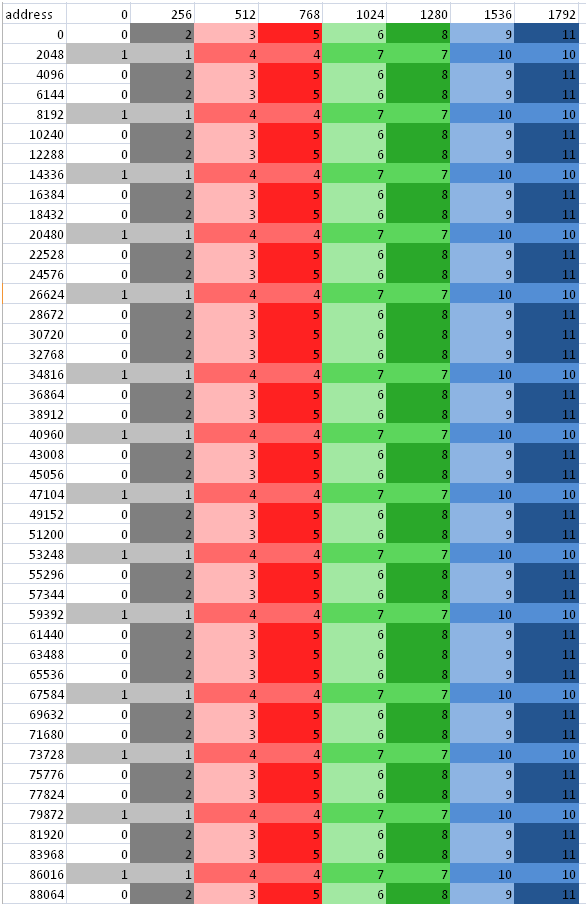
\includegraphics[width=0.50\textwidth]{gpu_mem_channel}
	\bicaption{AMD GPU channel分布}{AMD GPU memory channel distribution}
	\label{fig:gpu_mem_channel}
\end{figure}

可以根据图\ref{fig:gpu_mem_channel}得到,如果访存步长是2048,那么将会有1/3的概率会访问到相同的channel;如果的访存步长是256,那么将会有1/6的概率访问相同的channel。

\section{GPU微体系结构}
\subsection{NVIDIA GPU架构}
NVIDIA GPUs由许多SMs(Streaming Multiprocessor)构成。每个SM包含多个SPs(Streaming Processor)(每个SP是基本的计算单元),调度器,和SFUs(Specital Functional Unit),LD/ST(Load/Store)单元,寄存器文件和统一共享内存/L1 cache。一个SM中的SPs共享寄存器文件和shared memory。NVIDIA GTX280,GTX580和GTX680三代GPU的比较(如图\ref{fig:nvidia_3_gpus})
\begin{figure}[htbp]
	\centering
	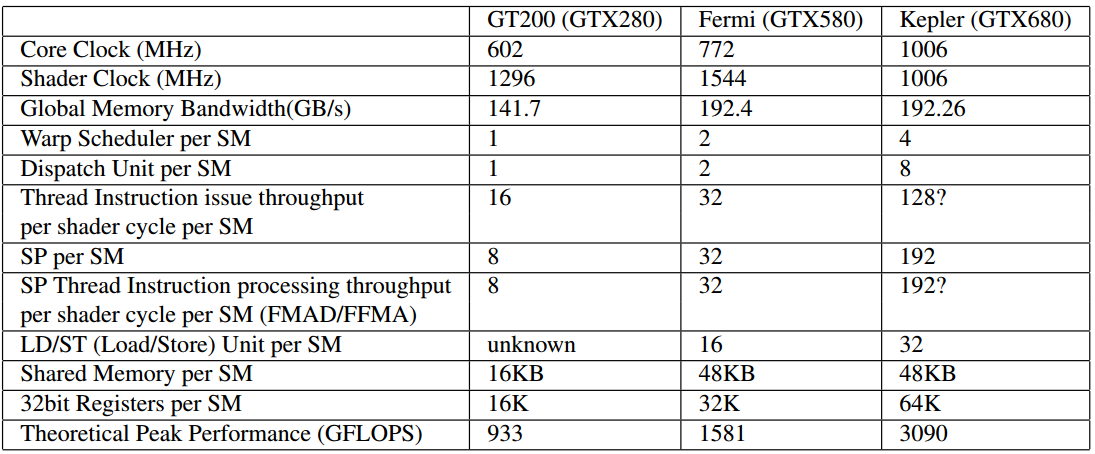
\includegraphics[width=0.80\textwidth]{nvidia_3_gpus}
	\bicaption{NVIDIA三代GPU的比较}{Comparison of NVIDIA Three Gen. GPUs}
	\label{fig:nvidia_3_gpus}
\end{figure}
从GT200到Kepler,SP(Streaming Processor)的数量急剧增长。从240(GTX280,65nm)到1536(GTX680,28nm)。然而,当我们从一个SP的角度来看,每个SP拥有的寄存器和shared memory这样的片上内存资源其实在变少。在Kepler(GTX680)之前的GPU,每个SM有两个时钟域:调度器的时钟core clock和SPs的时钟shader clock。Shader clock的频率大致是core clock的两倍。Kepler(GK104)之后,去掉了shader clock,一个SM的所有功能单元使用同一个时钟。为了便于比较不同的GPU架构,我们在Kepler GPU仍然沿用shader clock术语。

一个典型的CUDA程序通常会创建几千个并发线程来掩盖访存延迟和流水线延迟。线程的组织方式为,多个线程组成一个block,多个block再组成一个grid。一个Warp由32个线程组成,是SM上基本的执行和调度单元。我们将一个warp中所有线程执行的指令称为warp指令,将单个线程执行的指令称为thread指令。所以,一个warp指令包含32个thread指令。

在一个SM中,只有有限个线程可以并发的执行,称为active线程。一方面,一个SM中SPs越多,我们就需要更多的active线程来掩盖延迟。但另一方面,SM中的寄存器的数量和shared memory的大小等硬件资源又会限制SM中active线程的数量。从Fermi GPU到Kepler GPU每个SP可用的寄存器数量和shared memory大小在变少,因此单个SP支持的active线程数在减少。对于Fermi和Kepler GK104指令级,每个线程可用63个寄存器。因为在指令编码中,编码寄存器的段为6 bit。

\subsection{AMD GPU微架构}
 AMD GPU计算部件由多个Compute Unit(计算单元)组成,对应于NVIDIA的SM(Streaming Multi-processor), (从SIMD0$\sim$SIMD3)四个SIMD构成一个Compute Unit。每个SIMD有自己40-bit的程序计数器,和10个wavefronts(对应NVIDIA的warp)的指令缓存。一个Compute Unit(计算单元)可以最多可同时运行40个wavefronts,每个SIMD最多有10个wavefronts。Vega10 GPU增加了半精度浮点运算部件。



\subsubsection{AMD GCN Data Parellel Processor阵列结构}
 AMD GCN处理器是一种并行微架构,不仅可用于计算机图形应用,而且也可用于通用数据并行应用。任何需要高带宽或计算密集型的数据密集型应用程序都可以在AMD GCN处理器上运行。图\ref{fig:amd_vega_arch}展示了AMD Vega GPU内部结构。
 
 GCN架构包括数据并行处理器(DPP Data Parallel Processer)阵列,命令处理器,存储器控制器和其他逻辑。GCN命令处理器读取主机写入系统内存地址空间中的命令。当命令完成时,命令处理器将硬件生成的中断发送给主机端。 GCN内存控制器可直接访问所有GCN设备内存和主机指定的系统内存区域。存储器控制器使用DMA的方式进行数据的读取和写入。
 
 在GCN结构中,一个完整的应用程序包括两部分:
 
(1) 在主机端运行的程序。
 
(2)在GCN处理器上运行的程序,称之为kernel。
 
\begin{figure}[htbp]
	\centering
	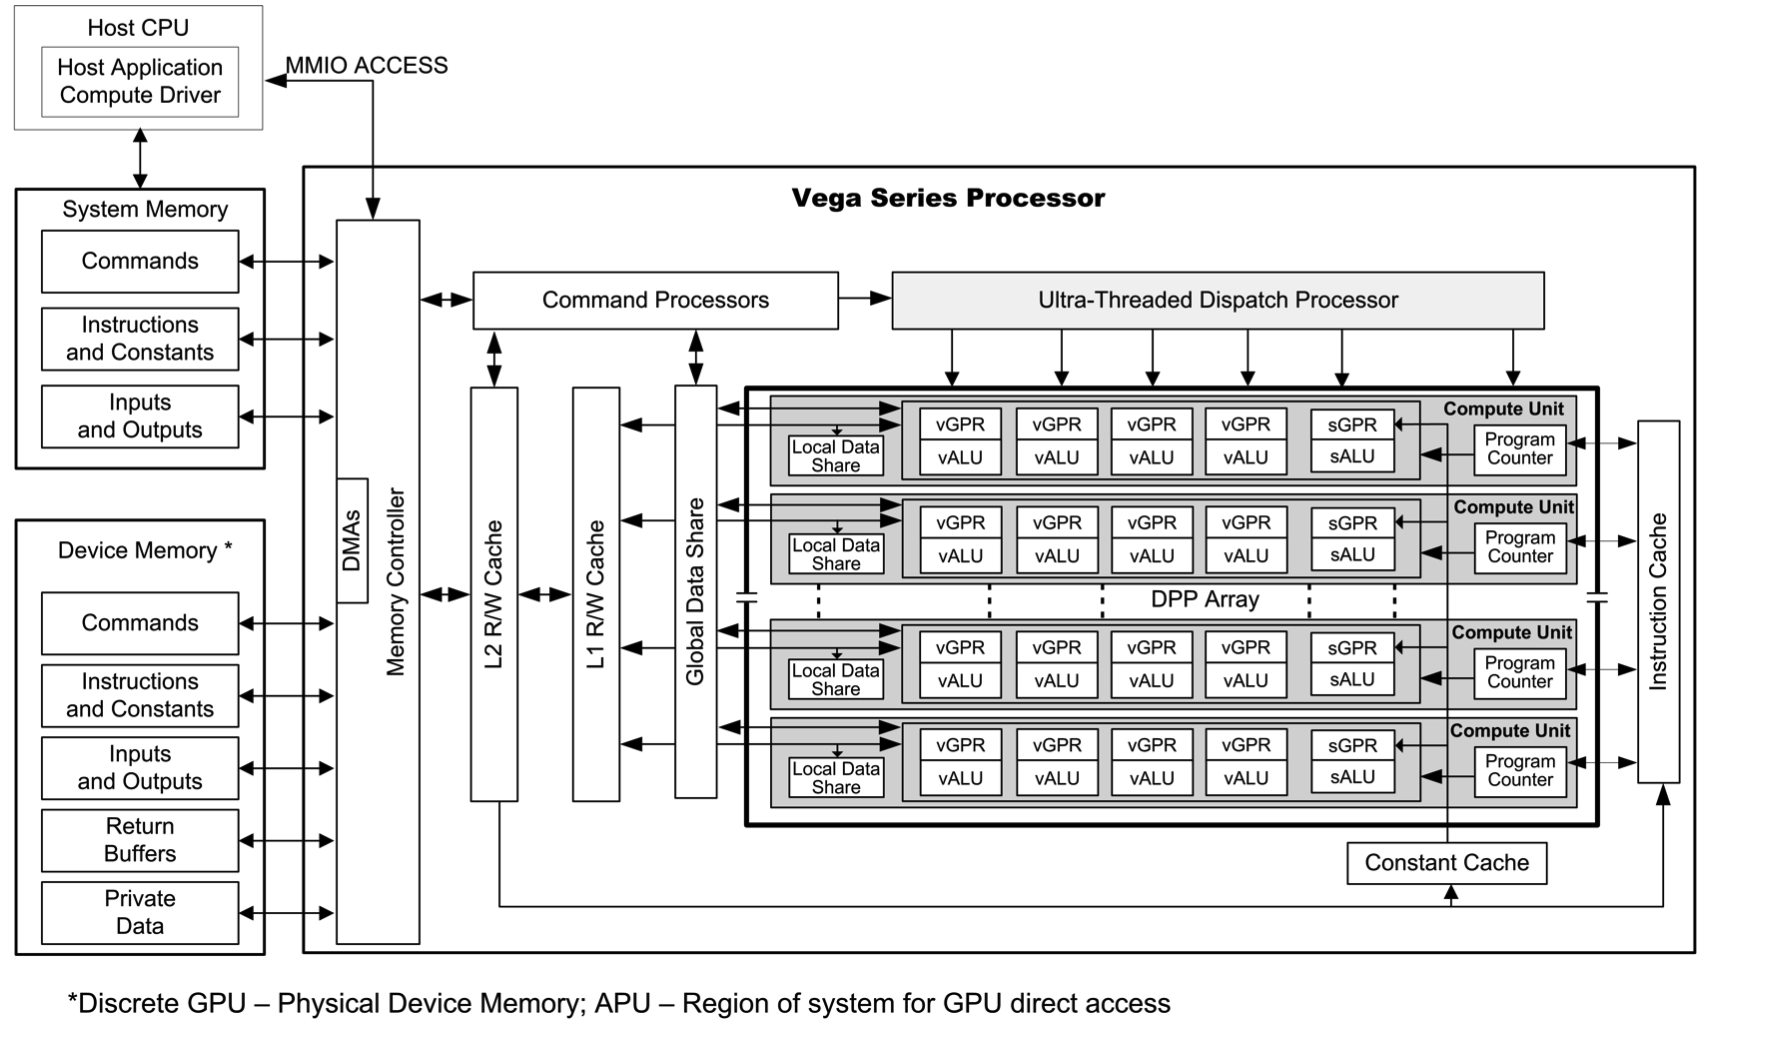
\includegraphics[width=0.80\textwidth]{amd_vega_arch}
	\bicaption{AMD VEGA GPU结构图}{AMD VEGA architecture}
	\label{fig:amd_vega_arch}
\end{figure}

GCN程序由主机命令控制,包括:

(1) 设置GCN内部基址和其他配置寄存器。

(2) 指定GCN GPU要在其上运行的数据域。

(3) 发送命令让GCN GPU开始执行程序。
%
%GCN驱动程序在主机上运行。
%
%DPP阵列是GCN处理器的核心。该数组被组织为一组计算单元流水线,每个流水线独立于其他计算单元流水线,并行运行在浮点部件或整数部件上。计算单元流水线可以处理数据,或通过内存控制器将数据传输到内存或从内存传输数据。当DPP接收到一个请求时,计算单元管道从内存加载指令和数据,开始执行,直到内核结束。内核正在运行时,GCN硬件会自动将指令从内存提取到片上高速缓存中; GCN软件在这方面没有任何作用。GCN内核可以将数据从片外存储器加载到片上通用寄存器(GPR)和高速缓存中。
%
%AMD GCN硬件可以检测浮点异常并生成中断。 特别是,他们在硬件中检测IEEE浮点异常; 这些可以被记录用于执行后分析。 上图中从命令处理器到主机的软件中断代表硬件生成的用于信号命令完成和相关管理功能的中断。
%
%GCN处理器通过跟踪潜在的数百个work-item的不同执行阶段,以及将计算操作与内存访问操作进行重叠来隐藏内存延迟。
%
%DPP阵列是GCN处理器的核心。该数组被组织为一组计算单元流水线,每个流水线独立于其他计算单元流水线,并行运行在浮点部件或整数部件上。计算单元流水线可以处理数据,或通过内存控制器将数据传输到内存或从内存传输数据。当DPP接收到一个请求时,计算单元管道从内存加载指令和数据,开始执行,直到内核结束。内核正在运行时,GCN硬件会自动将指令从内存提取到片上高速缓存中; GCN软件在这方面没有任何作用。GCN内核可以将数据从片外存储器加载到片上通用寄存器(GPR)和高速缓存中。
%
%AMD GCN硬件可以检测浮点异常并生成中断。 特别是,他们在硬件中检测IEEE浮点异常; 这些可以被记录用于执行后分析。 上图中从命令处理器到主机的软件中断代表硬件生成的用于信号命令完成和相关管理功能的中断。

GCN处理器通过跟踪大量work-item的不同执行阶段,通过线程间切换,将计算操作与内存访问操作进行重叠来隐藏访存延迟。
图\ref{fig:amd_cs}展示了GCN应用程序的数据流动。
\begin{figure}[htbp]
	\centering
	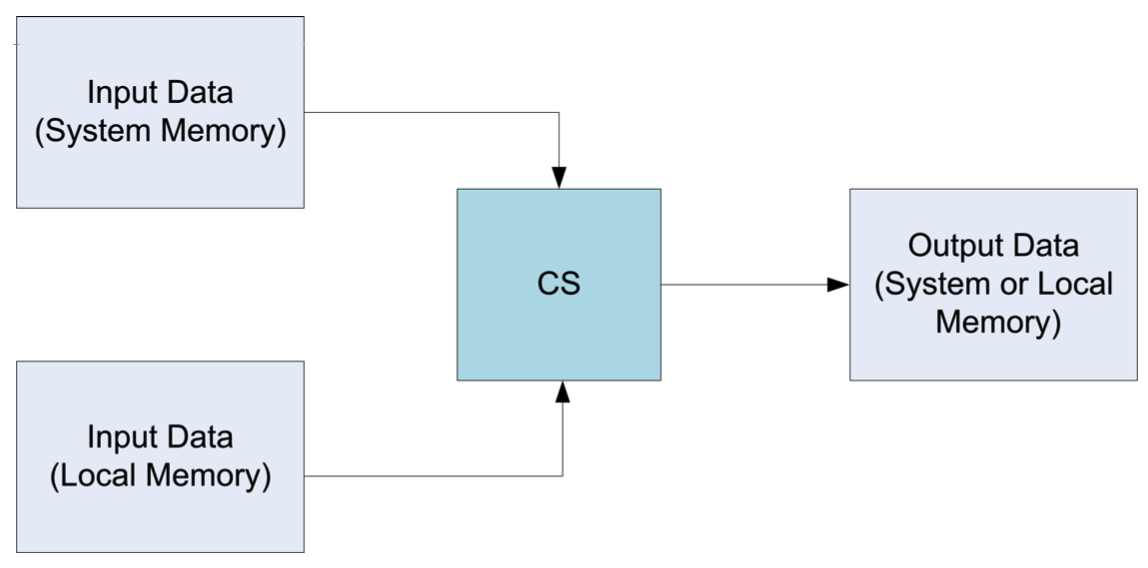
\includegraphics[width=0.50\textwidth]{amd_cs}
	\bicaption{GCN GPU程序数据流动}{GCN GPU program data flow diagram}
	\label{fig:amd_cs}
\end{figure}

GCN kernel是由GCN处理器执行的程序。从概念上讲,kernel在每个work-item上都是独立执行的,但实际上GCN处理器将64个work-item分组到一个wavefront中,wavefront并行执行所有64个work-item的指令。

GCN处理器由以下部分组成:

(1) 一个标量ALU,为一个CU的所有work-item所共用。

(2)	4个向量ALU,向量ALU的宽度为16,一个work-item在其中的一个lane中执行。

(3) 一个Local Data Share,使得workgroup中的work-item可以进行通信和数据共享。

(4) 标量访存部件,可以通过Cache在SGPR和内存之间传输数据。

(5) 向量访存部件,可以在VGPR和存储器之间传输数据。

%所有内核控制流都使用标量ALU指令处理。这包括if / else,分支和循环。标量ALU(SALU)和访存指令适用于整个wavefront。向量访存和ALU指令一次对wavefront的所有work-itme进行操作。为了支持分支和条件执行,每个wavefront都有一个EXECUTE掩码,用于确定哪些work-item在当时处于活动状态,哪些处于休眠状态。活动的work-item执行矢量指令,休眠的work-item将该指令视为NOP。可以随时通过Scalar ALU指令更改EXEC掩码。向量访存指令在VGPR和存储器之间传输数据。每个work-item都提供自己的内存地址并提供或接收唯一的数据。这些也受到EXEC掩码的约束。
\subsubsection{AMD GPU内存层次结构}
AMD GCN流处理器可以在不同的work-item之间共享数据。数据共享可以显著提升性能。图\ref{fig:amd_gpu_memory}展示了AMD GCN处理器内存层次结构。
\begin{figure}[htbp]
	\centering
	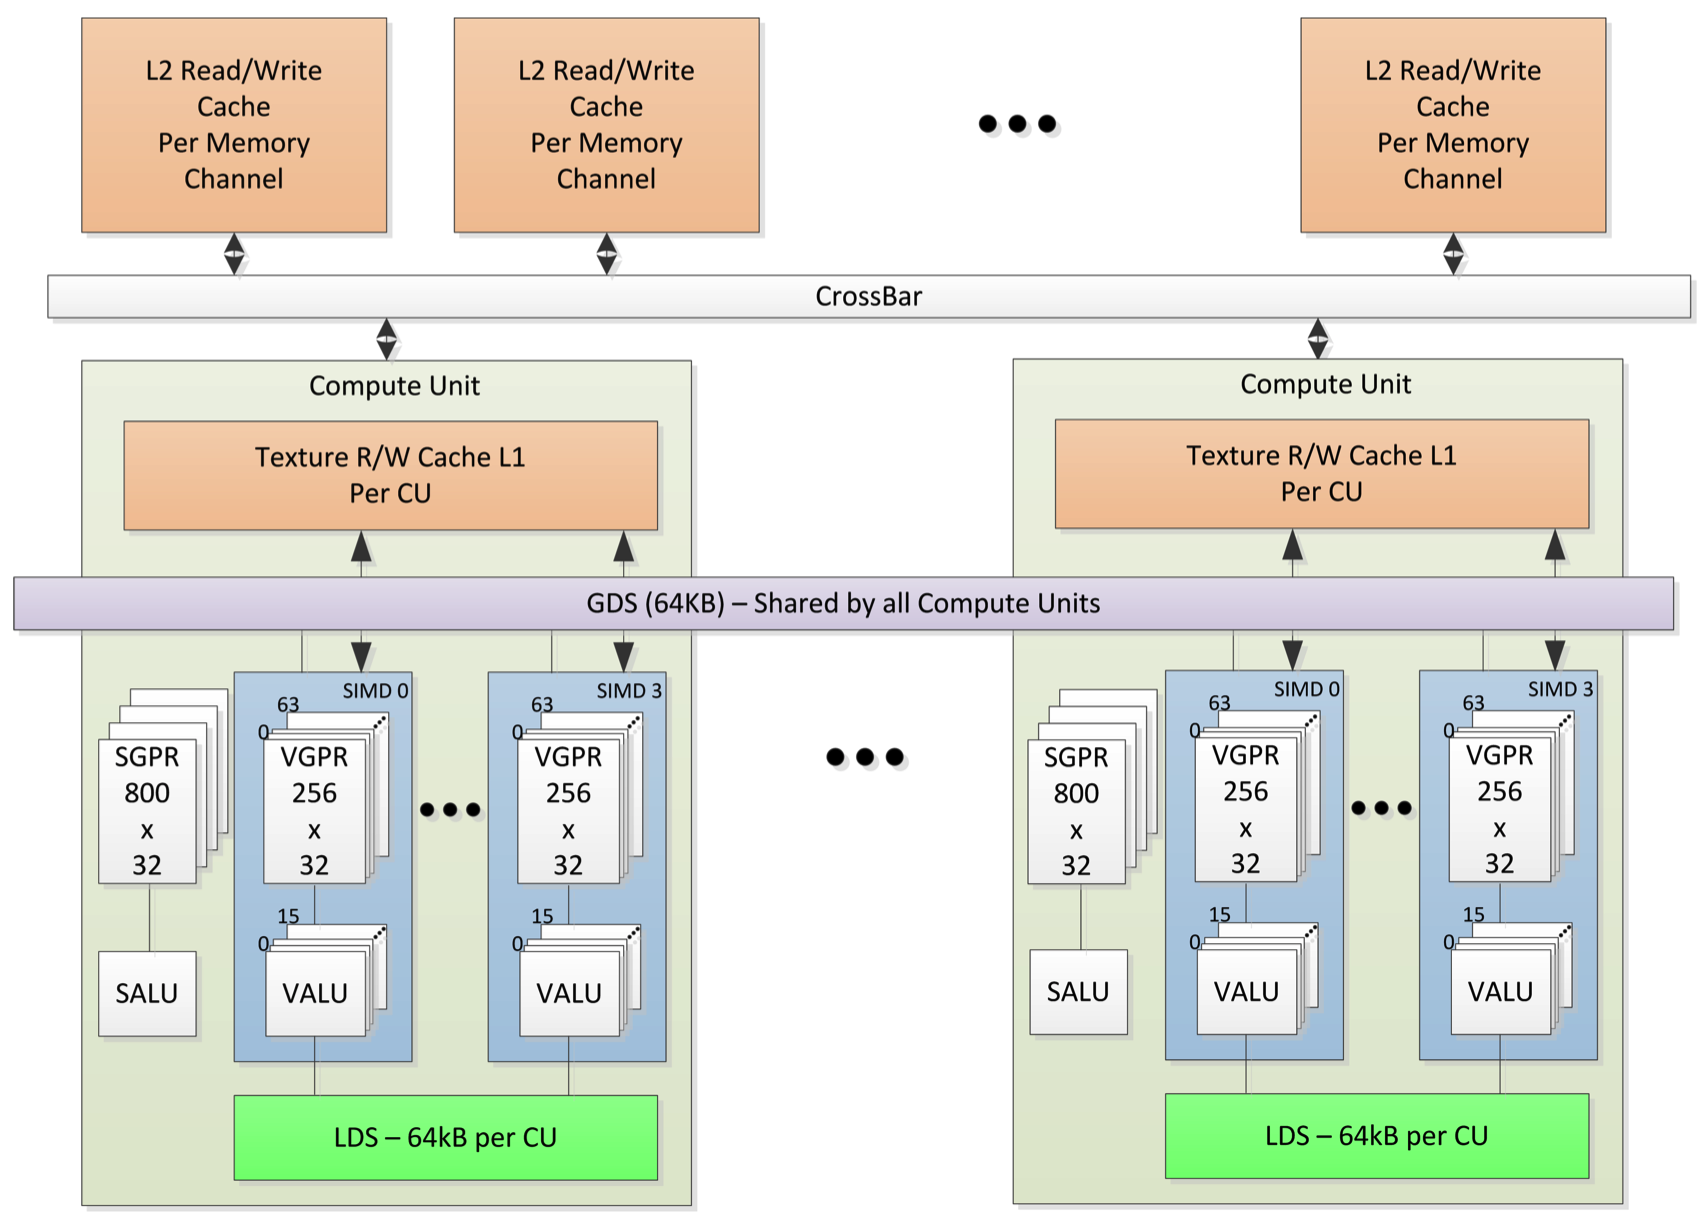
\includegraphics[width=0.80\textwidth]{amd_gpu_memory}
	\bicaption{AMD GPU内存层次结构}{AMD GPU memory hierarchy}
	\label{fig:amd_gpu_memory}
\end{figure}
每个CU都有一个64kB的片上内存LDS(Local Data Share),可以实现一个work-group中不同work-item或一个wavefront中不同work-item之间的低延迟通信。每个LDS有32个banks,每个bank的宽度为4字节。AMD GCN处理器的每个CU有64kB LDS,为其提供了64kB的片上低延迟带宽。


\subsection{AMD GPU和NVIDIA GPU架构的比较}
在计算单元的设计上,AMD和NVIDIA GPU的计算单元都采用了SIMD(Single Instruction Multiple Data)或者SIMT(Single Instruction Mulitiple Thread)架构。在术语上,AMD称其为SIMD,NVIDIA称其为SIMT或SPMD(Single Program Multiple Data)。AMD GPU由很多CU(Compute Units)组成,NVIDIA GPU由很多SM(Streaming Multi-processors)或SMX组成。对于AMD Redeon Vega10架构,每个CU有4个SIMD部件,每个SIMD的宽度为16。通过向量流水线的方式用4个时钟周期来执行宽度为64的向量操作。对于NVIDIA GTX780,其设计为Kepler架构,每个SMX有12个SIMD,每个SIMD的宽度为16。通过2个时钟周期来执行宽度为32的向量操作。

对于AMD GPU GCN架构,每个CU包含一个标量部件和4个SIMD部件,每个SIMD最多可以有10个向量线程(AMD称为wavefronts)in flight,向量线程的宽度为64。一个SIMD在每个指令发射周期选择一个向量线程来执行。所以,一个CU最多可以运行40个向量线程。NVIDIA GPU在设计上也与之类似。但实际可运行的向量线程数受很多因素限制,这里包括寄存器数量,局部共享内存的大小等。

对于AMD GPU和NVIDIA GPU体系结构,采用了SIMD的编程模型,每个线程是SIMD中的一项。NVIDIA称之为“SIMT(Single Instruction, Multiple Thread)”或者“SPMD(Single Program, Multiple Data)”。对于AMD GPU,一个wavefront有一个程序计数器,指令的分支由专门的寄存器做掩码来标记,控制每个线程的行为。

通过上面的比较,我们可以看出,AMD GPU和NVIDIA GPU都采用了SIMD结构,不同的是AMD GPU所计算的向量的宽度为64,NVIDIA GPU所计算的向量宽度为32。由此可以窥见SIMD结构代表着现代GPU的主流设计方向。

对于AMD GPU GCN架构,每个CU包含一个标量部件和4个SIMD部件,每个SIMD最多可以有10个向量线程(AMD称为wavefronts)in flight,向量线程的宽度为64。一个SIMD在每个指令发射周期选择一个向量线程来执行。所以,一个CU最多可以运行40个向量线程。NVIDIA GPU在设计上也与之类似。但实际可运行的向量线程数受很多因素限制,这里包括寄存器数量,局部共享内存的大小等。

GPU上的指令级并行。对于AMD GPU每个时钟周期可发射多条向量指令,每个向量指令将被分发到不同的向量单元。AMD GPU的指令可以超标量执行,在同一个CU上,可以同时执行访存指令,计算指令和其他占用不同部件的操作。这样可以提高GPU执行指令的通量。AMD Radeon R9 290X有44个CUs,每个CU包含4个向量单元,共176个向量单元。NVIDIA GeForce GTX 780有12个SMX,每个SMX有12个向量单元,共144个向量单元。这两种GPU都有高速片上内存,在OpenCL的术语中,称之为局部内存。以一个线程块(work-group)为单位进行分配。

相比于CPU中线程的概念,GPU中的线程非常轻量级,可以做非常快速的线程切换。GPU大量轻量级线程的特点,使其可多任务快速切换和实现高吞吐量。线程的运行上,GPU会简单很多,是顺序发射,没有CPU中线程的多发射和乱序执行。由于GPU有大量向量部件,通过产生大量轻型线程来充分利用这些部件。所以,GPU是面向通量计算的处理器。


\section{AMD GPU微基准测试}
根据AMD GPU微结构的特点,设计出了一个微基准测试程序。通过微基准测试程序,可以探测AMD GPU的指令通量和内存带宽。


\subsubsection{AMD GPU指令通量和带宽探测}
\begin{figure}[htbp]
	\centering
	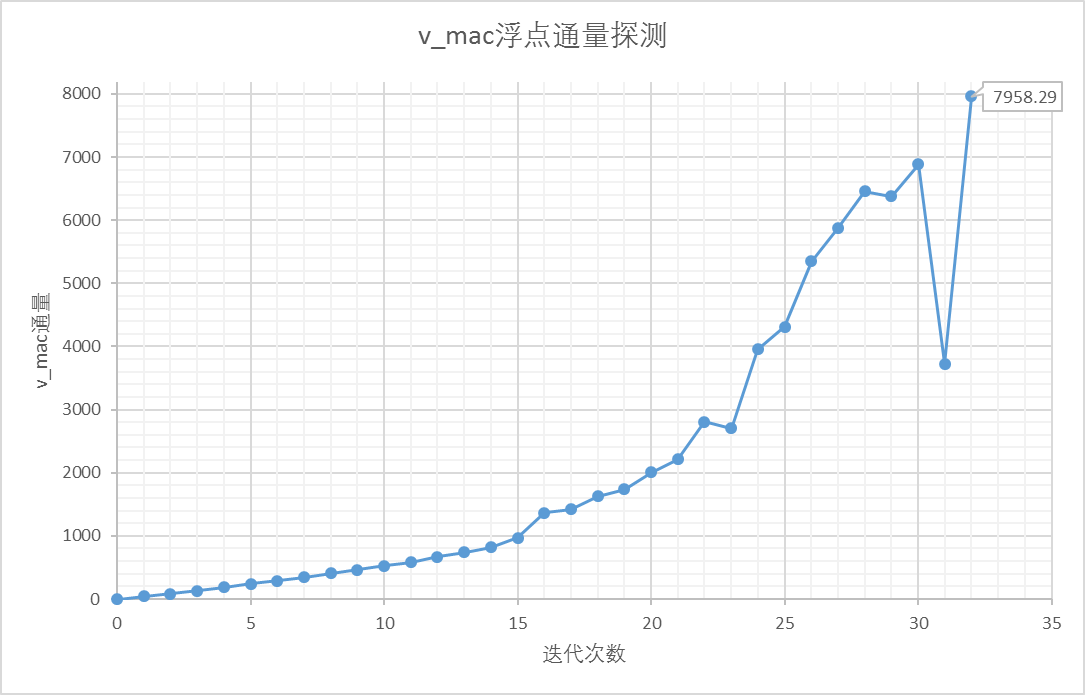
\includegraphics[width=0.50\textwidth]{v_mac_throughput}
	\bicaption{AMD Fiji GPU浮点通量测试}{AMD Fiji GPU floating point throughput}
	\label{fig:v_mac_throughput}
\end{figure}

探测得的AMD Fiji R9 Nano GPU的浮点通量为7958.29gflop/s。Fiji GPU的理论浮点峰值为8192gflop/s,所以实测浮点性能为7958.29/8192 = 97.15\%。

\begin{figure}[htbp]
	\centering
	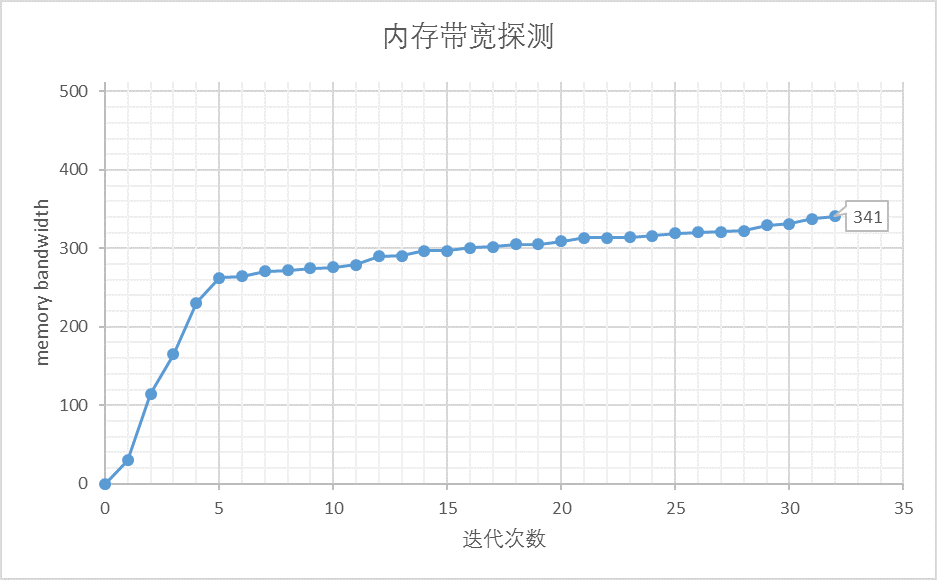
\includegraphics[width=0.50\textwidth]{mem_bandwidth}
	\bicaption{AMD Fiji GPU内存带宽测试}{AMD GPU memory hierarchy}
	\label{fig:mem_bandwidth}
\end{figure}

探测得的AMD Fiji R9 Nano GPU的内存带宽为341GB/s。Fiji GPU的理论内存带宽为512GB/s,所以实测内存带宽为341/512 = 66.6\%。

\section{本章小结}
本章从GPU微体系结构和OpenCL编程模型两方面对AMD GPU架构进行了详细的描述。对比了AMD GPU和NVIDIA GPU在架构上的异同,观察出AMD和NVIDIA GPU在设计都采用了SIMD结构。两种GPU都通过并发大量轻型线程来做到延迟容忍,是面向通量计算的处理器。针对AMD GPU设计出一套微基准测试程序,探测出AMD GPU的浮点指令通量和内存带宽,为后面矩阵乘GPU调优做铺垫。


